\chapter{Perspectives}
The different perspectives will be presented and following in this chapter is a more thorough examination of how the different perspectives are related, how one perspective translates to another, the transition between them, and which perspectives fits which purposes.


\section{The Different Perspectives}
There are a lot of different ways that news can be presented, considering how much information from a news article that are shown, how it is shown graphically, what the information shown means in different contexts etc. Following are description of the perspectives that are most used in different news applications and the applications referred to in this section are examined and presented in section \ref{commercial_news_applications}.

\subsubsection{Full Article}
A full article perspective, as the name implies, is perspective that normally holds all the information available for that particular news story. The most important information in this perspective is the full article text, as this is the information that most often is lacking in the other perspectives. Figure \ref{full_article_prismatic} shows an example of a full article perspective.

\begin{figure}[!htbp]
\centering
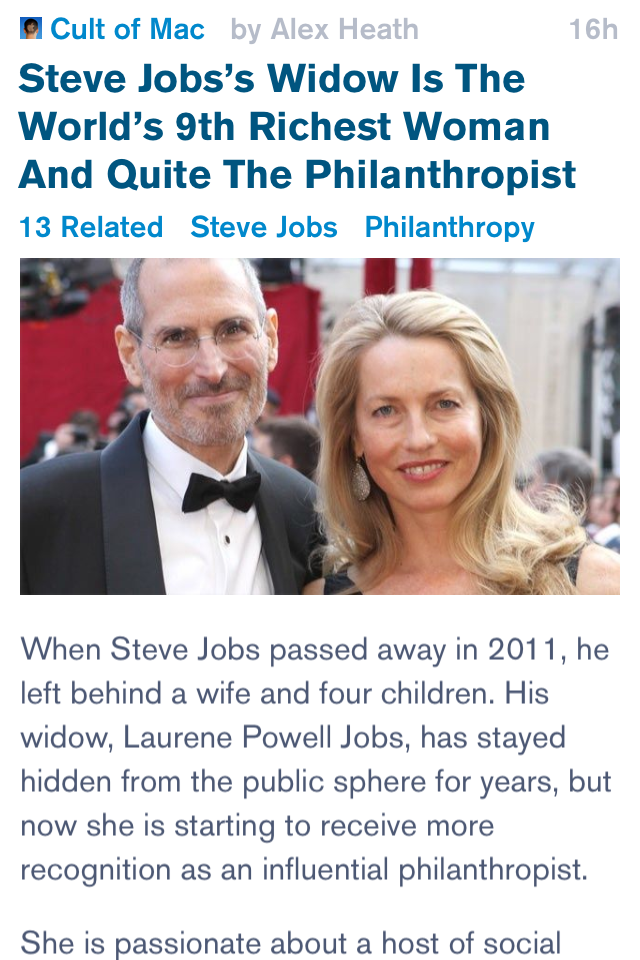
\includegraphics[width=50mm]{GFX/perspectives/fullArticleViewPrismatic.png}
\caption{A screenshot from Prismatic showing an example of a full article perspective.}
\label{full_article_prismatic}
\end{figure}

\subsubsection{RSS}
An RSS perspective is a perspective showing just some of the information from an article to give the user a quick overview of what the news article concerns. The name stems from the RSS feed technology which has a certain set of information like title, lead-text, when the article was published, and sometimes an image. The RSS view may have other information as well, but the ones mentioned are the most common. Figure \ref{rss_feedly} shows an example of how an RSS perspective may be presented.

\begin{figure}[!htbp]
\centering
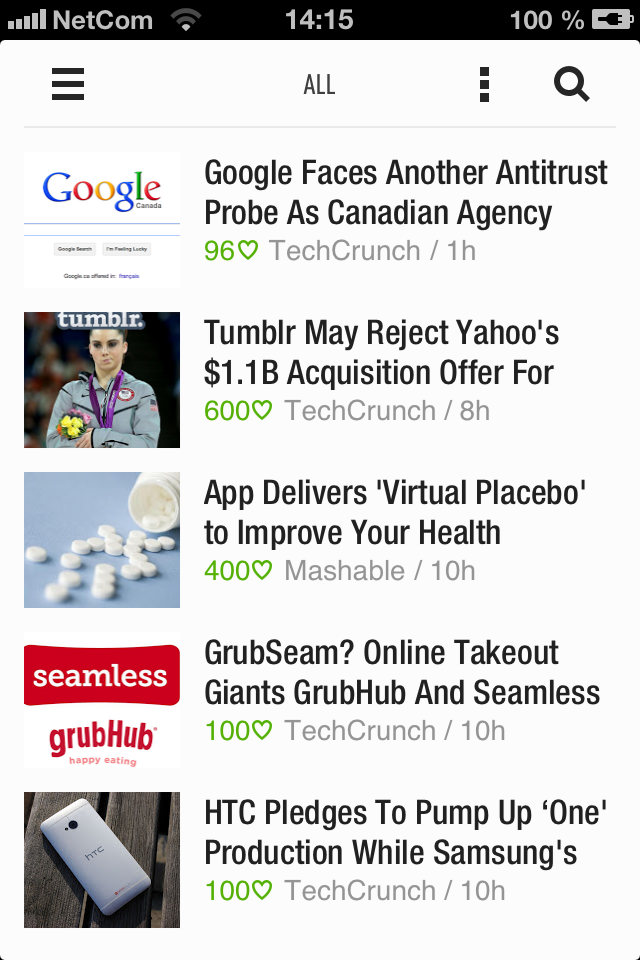
\includegraphics[width=50mm]{GFX/perspectives/rssViewFeedly.png}
\caption{A screenshot from Feedly showing an example of an RSS perspective.}
\label{rss_feedly}
\end{figure}

\subsubsection{Entity}
An entity perspective is a perspective showing a set of keywords extracted from a news article by the use of a keyword extracting algorithm or other NLP technologies. Figure \ref{entity_news_cloud} shows an example of how an entity perspective can be displayed to the user. In this application if a keyword is selected, all the other keywords that are connected to this keyword is highlighted. The articles these keywords are extracted from are shown in a view on the right-hand side as links that will take the user to the corresponding article if clicked.

\begin{figure}[!htbp]
\centering
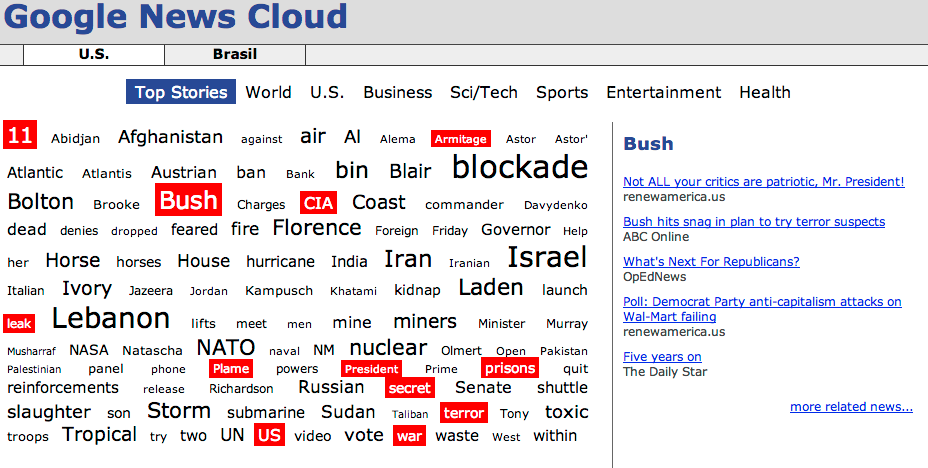
\includegraphics[width=140mm]{GFX/perspectives/entityViewNewsCloud.png}
\caption{A screenshot from NewsCloud showing an example of an entity perspective.}
\label{entity_news_cloud}
\end{figure}

\subsubsection{Event}
An event perspective is a perspective that displays certain events that occurred by analyzing news articles and extracting those events by using NLP or other text-analyzing techniques. Figure \ref{event_wavii} shows three events extracted from different news articles. The first shows that two celebrities broke up, the second shows that a theatrical trailer was released by a movie publisher and the third shows that a software company released a new application for the iOS platform.

\begin{figure}[!htbp]
\centering
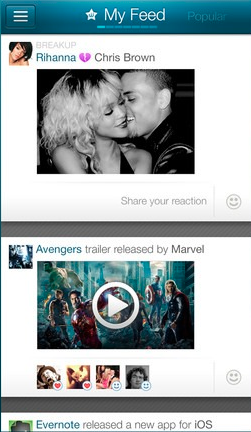
\includegraphics[width=50mm]{GFX/perspectives/eventViewWavii.png}
\caption{A screenshot from Wavii showing an example of an event perspective.}
\label{event_wavii}
\end{figure}

\subsubsection{Web}
The web perspective is quite similar to the full article perspective and usually includes the same amount of information. The main difference is that the web perspective is the news article shown at the publisher's website through an application by the use of a web browser inside a third party application. This is a widely used perspective as a third party application cannot normally show a full news article from another publisher without an agreement with the publisher itself. Showing a full article without a contract with the publisher is most likely a copyright infringement. Figure \ref{web_flipboard} shows an example of how a web perspective may be presented.

\begin{figure}[!htbp]
\centering
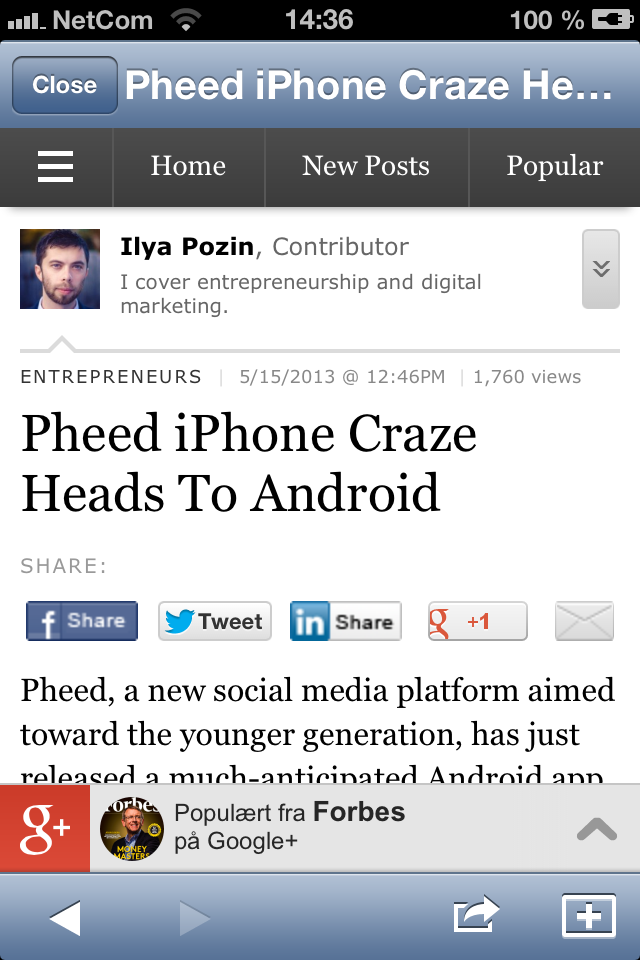
\includegraphics[width=50mm]{GFX/perspectives/webViewFlipboard.png}
\caption{A screenshot from Flipboard showing an example of a web perspective.}
\label{web_flipboard}
\end{figure}

\subsubsection{Summary}
The summary perspective is a perspective that shows a summary text of the full article text, where this text is created by the use of NLP technologies, like the Summly application, or hand crafted by real editors, like the Circa application. Figure \ref{summary_summly} shows a screenshot of the Summly application presenting a summary perspective.

\begin{figure}[!htbp]
\centering
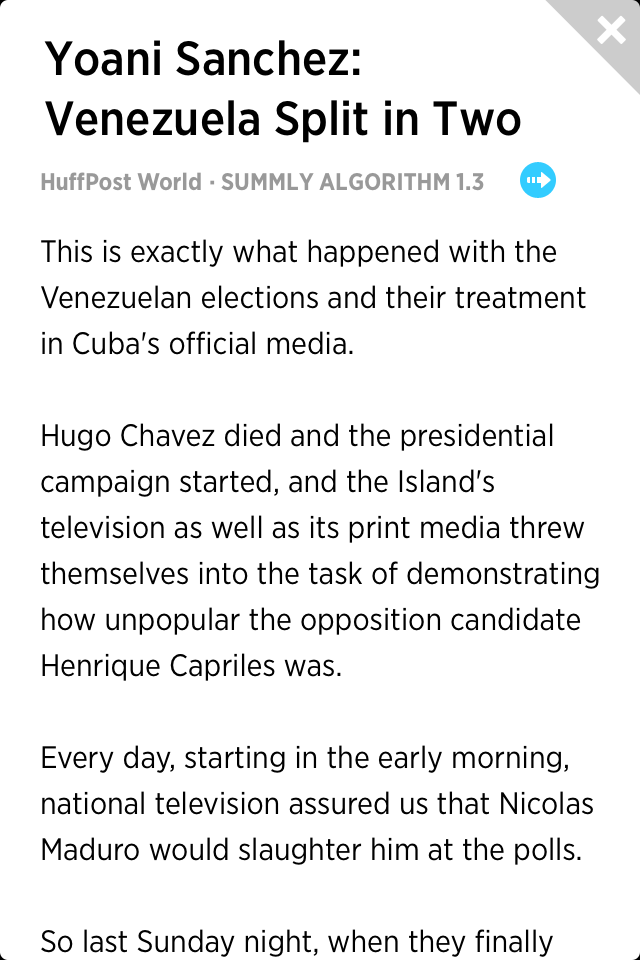
\includegraphics[width=50mm]{GFX/perspectives/summaryViewSummly.png}
\caption{A screenshot from Summly showing an example of a summary perspective.}
\label{summary_summly}
\end{figure}

\subsubsection{Map}
The map perspective is a perspective that shows where in the world a news story concerns by the use of a map view. Figure \ref{map_circa} shows a news story residing in Lisbon, Portugal in the Circa application.

\begin{figure}[!htbp]
\centering
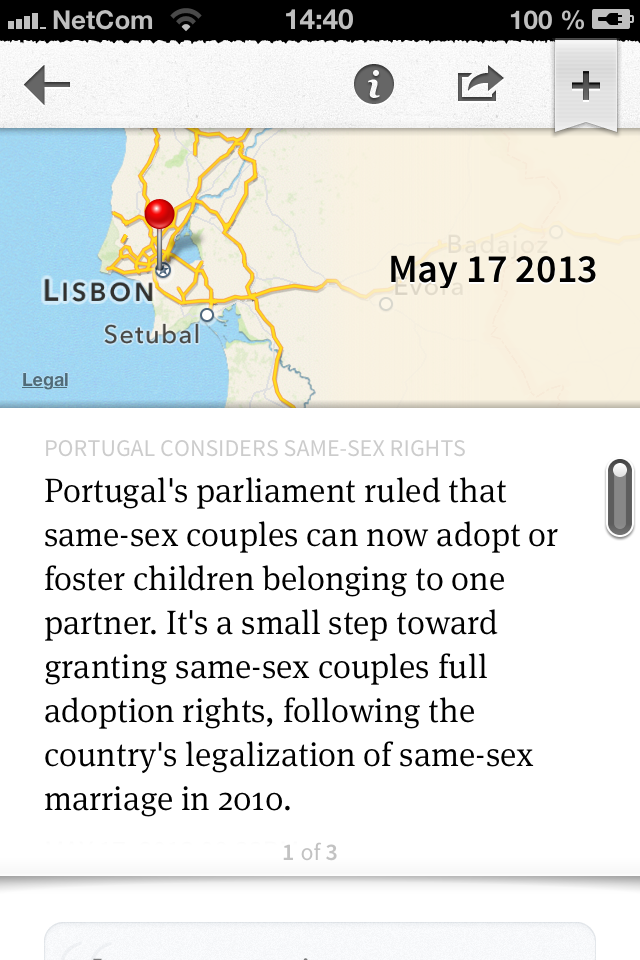
\includegraphics[width=50mm]{GFX/perspectives/mapViewCirca.png}
\caption{A screenshot from Circa showing an example of a map perspective.}
\label{map_circa}
\end{figure}

\section{Relations}
A perspective can present all the information available from a news article or just a subset of the information, depending on which purpose the perspective has and what type of information the perspective is trying to convey. Following is an explanation of how the different perspectives are related.

\subsubsection{Full Article Perspective and Web Perspective}
The full article perspective and the web perspective are the two perspectives that holds the most information and are most related. The main difference between the two is that the full article perspectives presents its information in a native way, following the UI design that goes with rest of the application, while the web perspective is presented as a web page in a web browser wrapper inside the native application. The full article perspective is designed by the creator of the native application, while the web perspective usually is designed by the content publisher itself as a responsive web page\footnote{A responsive web page is web page that adapts to the screen size and resolution of the device opening the web page.}. If a native app developer wants to show all information available from a news article, it usually has to be done via a web perspective to avoid copyright infringement. The developer can present it as a full article perspective if the app developer has some kind of agreement with content publisher who has the copyright, or the app developer is the content publisher itself.

\subsubsection{RSS Perspective}
All the other perspectives presents information that can somehow be derived from the full article perspective or the web perspective. The RSS perspective normally holds the information that are available from an RSS feed, hence the name, which is information that usually are available and free to use from the content publishers itself, as long as it links to the web perspective of the same article.

\subsubsection{Entity Perspective}
The entity perspective holds information in terms of keywords. Normally these keywords are not available from any content supplier, but has been processed from the news article's title, lead text, and full article text, by the use of some sort of keyword extraction algorithm or other NLP technologies. For the best result the event perspective is derived from the full article perspective or web perspective to be able to process all of the information available, but it can also be derived from the RSS perspective, as the title and lead text alone often holds important keywords that are sufficient to understand what the articles comprises.

\subsubsection{Event Perspective}
Similar to the entity perspective, the event perspective holds information that are derived and processed from the full article perspective or the web perspective. To extract the information shown in the event perspective, advanced NLP technology needs to be applied and a deeper understanding of the article needs to be established. Deriving information from the RSS perspective is most likely not sufficient to overcome this. An event may be extracted from the RSS perspective, but titles and lead texts alone may be misleading or not convey fully what the full story text tries to communicate.

\subsubsection{Summary Perspective}
NLP is a fairly important domain when processing news articles and extracting useful information, and the summary perspective is another example of just this. As the name implies, the summary perspective most often shows a summary of the full article text derived from the full article perspective or web perspective. The summaries can be created by the use of NLP, like the Summly application, or by real editors like the Circa application. The summary perspective are not limited to a text summary, it can also hold information from the entity perspective and the event perspective as these also are a form of summaries or compressed information from the full article perspective or web perspective.

\subsubsection{Map Perspective}
To be able to show on a map where news articles resides, the information from the full article perspective or web perspective needs to be thoroughly processed and analyzed, and again NLP is an important part of this. Places can be extracted from the title, lead text or the full article text, but this information is not sufficient to say where an article's content concerns. There are several challenges to overcome to accomplish an accurate map perspective. 

The name of a place without knowing the coordinates of the place, can point to several places throughout the globe. For instance, Heimdal is a place near Trondheim, Norway, but is also a place in North Dakota, USA. To be able to pick the right one, a deeper understanding of the article is necessary. 

Also an article can mention several places in the full article text, without all of these places necessarily concerns the article itself. For instance, the article can state "The rock and roll band Aerosmith from Boston, Massachusetts is playing the O2 arena in London next week, with support from the electronica band Röyksopp from Tromsø, Norway". In this example London would be the place the article concerns, and Boston and Tromsø are places that would be misleading to pin to a map with same significance as London.


\section{Purpose of and Flow between Perspectives}
The different perspectives serves different purposes, and have various areas of usage. Following are a description of the perspectives' main functions and where they convey their information to the fullest, ordered after when they are most likely to appear to the user. The more information the perspective can hold the farther down in the navigation hierarchy they are likely to be.


\subsubsection{RSS Perspective}
The RSS perspective often serves as an entry point to a news article and its purpose is to give a quick overview of the content of the article and/or to trigger a curiosity at the user's end to make them wanting to read more. The information in the RSS perspective are often authored by a journalist from the content publisher to achieve exactly this purpose, to drive more traffic to the content publisher's web page, which again will give the content publisher more advertising revenue. With this in mind the RSS perspective is on a thin line between supplying enough information to give the user an understanding of what the topic and main content of the article is, but at the same time create enough curiosity to make the user wanting to read more.

\subsubsection{Summary Perspective}
The summary perspective is located somewhere in between the RSS perspective and the full article perspective or web perspective in the navigational hierarchy. For the users that want a little bit more information than what the RSS perspective can provide, but less than the full article perspective has to offer, it can serve as a replacement for both. It can work well as an entry point to an article and at the same time provide enough information to the user to make it satisfied with the information it has gained from the summary text. 

It can also serve as an additional level in the navigation hierarchy, between the RSS perspective and the full article perspective or web perspective, to give the user smaller steps between the perspectives and the amount of information presented.

\subsubsection{Event Perspective}
The event perspective shows important events extracted from the news article and is in a way a short summary consisting of the most important happenings in an article. For users browsing through many articles, this is a simple and efficient way to get the most important parts of an article. For these users an event perspective can work as an entry point to an article and replace the normally used RSS perspective. For some users the event perspective can also work as a replacement of the summary perspective, given that the events covers the essential content in the article. Similar to the summary perspective, the event perspective also can serve as an additional level in the navigation hierarchy to supply the user with some extra information in addition to the RSS perspective before deciding to navigate to the full article perspective.

\subsubsection{Entity Perspective}
The entity perspective can serve two main purposes. If presented as a supplemental perspective to the full article perspective or web perspective in the same level in the navigation hierarchy, it can serve as a way to find related articles and topics based on a news article. If, for instance, the entities in an entity view are "war, Bush, Al-Qaeda, Middle East, Iraq", these keywords can work as buttons to display a cluster of news about one of those keywords, or they can be added to the user profile as an interesting topic to be included when recommending news articles.

On the other hand, the entity view can serve as a way of getting a quick overview of what the main topics of an article are and then decide to go further into the navigation hierarchy to read more about it. Considering the example given over, a user can easily decide if this is a topic worth reading more about, or skip through. With this approach the entity perspective could replace the RSS perspective, and even the summary or event perspective for some users.


\subsubsection{Full Article Perspective}
The full article perspective has all the news article's information available, and are usually the last level in the navigation hierarchy. It is the perspective for the most interested users, who wants to have access to all the information an article has to offer, and to be able to read the whole story. This is a perspective primarily used by applications that have legal access to all the content of a story, like the content publishers themselves or third-party developers with special agreements with the content publishers.

\subsubsection{Web Perspective}
The web perspective serves the same purpose as the full article perspective, to satisfy the most interested users. This perspective are also usually located at the end of the navigation hierarchy, normally linked to from the RSS perspective, or one of the other perspectives that can replace the RSS perspective or work as a middle layer between the RSS perspective and web perspective, like the summary- event- or entity perspective.


\subsubsection{Map Perspective}
The map perspective has two main purposes. It can work as an additional perspective to the full article perspective or web perspective to show the user on a map where an article resides to provide the interested user even more information about the content.

It can also work as an entry point, but this can become a foul experience if not done right and then defeat its purpose. If used as an entry point, it would probably not be of much use to show a lot of articles spread out all over the world on a such small device, and have the user click every map pin to see if this could be an interesting story or not. On the other hand if the device can collect the users location and retrieve news that are nearby with coordinates that are accurate to where the news story concerns, the user can probably have a better understanding of the location, since the user is located nearby and probably knows the area better and can easier relate to the location. Then if a map pin is clicked the user can be brought further down in the navigation hierarchy.


\section{How the perspectives are supported on the mobile platform}
What APIs, hardware etc is used when applying these perspectives.